\documentclass[10pt]{article}
\usepackage[margin=1in]{geometry}
\usepackage{graphicx,amsmath,amssymb,booktabs,authblk,microtype}
\usepackage[dvipsnames]{xcolor}
\usepackage[numbers,sort&compress]{natbib}
\usepackage[colorlinks=true,allcolors=blue!55!black]{hyperref}
\graphicspath{{../results/figures/}}
\definecolor{navy}{HTML}{0b1f3a}
\renewcommand{\familydefault}{\sfdefault}
\title{\vspace{-2.2em}\textbf{\color{navy}\Large POLARIS: calibrated triangulation of non-coding\\[-1mm] variant evidence into mechanism and target gene}}
\author[1]{Aleksandar Stalevski}
\affil[1]{\small POLARIS Working Group $\cdot$ computational regulatory genomics}
\date{\vspace{-1.2em}\small\today}

\begin{document}
\maketitle
\vspace{-2.2em}

\begin{abstract}
\noindent Most disease-associated genetic variation is non-coding, and the field's central
obstacle is no longer prediction but \emph{principled integration}: powerful sequence oracles
disagree, are poorly calibrated, and degrade on distal and individual-level effects. We present
\textbf{POLARIS}, a transparent, calibrated framework that converts a disease's GWAS loci into
ranked, mechanistically-annotated causal-variant$\rightarrow$target-gene hypotheses while making
two long-standing guardrails mathematical. First, \emph{functional $\neq$ pathogenic}: POLARIS
factorizes the posterior into a molecular-function term and a disease-linkage term, and we show
empirically that allele rarity is \emph{inverted} for common-variant complex traits
(AUC $0.28$, $p=2\times10^{-3}$). Second, \emph{distrust any single oracle}: each evidence channel
is treated as a noisy annotator whose reliability is inferred by a Dawid--Skene-style latent-truth
EM, which autonomously learns that mammalian conservation is the most reliable molecular channel
(weight $0.62$) while transparent transcription-factor (TF) motif disruption is weak for variant
discrimination yet uniquely supplies mechanism. Applied to 30 type-2-diabetes (T2D) loci and
569 fine-mapped candidate variants, POLARIS recovers known effector genes at $85\%$ of textbook
control loci---its only failures being the canonical hard cases (distal \emph{FTO}$\rightarrow$\emph{IRX3},
imprinted \emph{DUSP8}), which its calibrated uncertainty correctly flags---and is well calibrated
(ECE $=0.005$). Its white-box biophysical module reproduces the textbook ARID5B$\rightarrow$IRX3
mechanism at \emph{FTO} rs1421085 from first principles ($\Delta$LLR $=-8.6$ bits), and a coupled
gene-regulatory ODE predicts the correct direction of effect. A random-matrix (Marchenko--Pastur)
analysis shows the evidence channels are largely independent, justifying triangulation. Critically,
\textbf{every finding replicates in an independent disease}---coronary artery disease (260 variants,
14 loci)---including the conservation enrichment, the rarity inversion, the inferred reliability
ordering, and recovery of the textbook \emph{SORT1} mechanism, with bootstrap-validated effect sizes
and a permutation-tested reliability inference ($p=0.01$). POLARIS is oracle-agnostic and fully
reproducible from public APIs, providing an auditable scaffold into which black-box predictors such
as AlphaGenome can be calibrated rather than trusted blindly.
\end{abstract}

\section{Introduction}
Genome-wide association studies (GWAS) implicate thousands of loci in complex disease, but
$\sim$90\% of lead variants are non-coding, acting through gene regulation rather than protein
sequence. Interpreting them requires traversing a noisy chain,
$\text{variant}\!\rightarrow\!\text{molecular effect}\!\rightarrow\!\text{gene}\!\rightarrow\!\text{tissue}\!\rightarrow\!\text{trait}$,
for which a rich toolbox now exists: statistical fine-mapping (SuSiE \citep{wang2020susie,zou2022susierss}),
sequence-to-function oracles (AlphaGenome \citep{avsec2025alphagenome}, Enformer \citep{avsec2021enformer},
Borzoi \citep{linder2025borzoi}), splicing predictors \citep{jaganathan2019spliceai,zeng2022pangolin},
deleteriousness scores \citep{rentzsch2021cadd}, colocalization \citep{giambartolomei2014coloc,wallace2021colocsusie},
and locus-to-gene models \citep{mountjoy2021l2g,gazal2022cs2g,flames2025}.

Yet these tools \emph{disagree}, and three failure modes recur. (i) The strongest oracles are
\emph{opaque}: AlphaGenome's developers caution that it captures distal elements ($>$100\,kb) poorly,
needs improvement on tissue specificity, and ``cannot fully explain how genetic variation leads to
complex disease'' \citep{avsec2025alphagenome}. (ii) Outputs are \emph{uncalibrated}: a high score is
not a probability of causation. (iii) Tools conflate \emph{molecular function} with \emph{disease
pathogenicity}, although a variant can perturb a regulatory element without contributing to a trait,
and---for polygenic traits---causal alleles are typically \emph{common}, not rare. The community's
working wisdom distils to two guardrails: \emph{functional $\neq$ pathogenic}, and \emph{triangulate;
distrust any single oracle}. These are stated as caveats but rarely operationalized.

POLARIS turns both guardrails into mathematics (Fig.~\ref{fig:pipeline}). It (1) factorizes the
disease-causal posterior so molecular function and disease linkage are separate, auditable terms;
(2) replaces black-box molecular prediction with a transparent, information-theoretic TF-binding
model whose every score is a calibrated log-odds with an exact $p$-value; (3) infers each channel's
reliability with a semi-supervised latent-truth model rather than hand-set weights; and (4) emits
calibrated posteriors with uncertainty that flags hard cases. We deliberately build POLARIS from a
\emph{fully transparent} oracle stack, demonstrating that auditable evidence---plus principled
integration---recovers textbook biology and is competitive with production tools, while remaining
oracle-agnostic so that black-box predictors can be \emph{ingested and calibrated} rather than trusted.

\section{Results}

\subsection{A transparent, reproducible pipeline for one disease}
We scope POLARIS to type-2 diabetes (T2D), which has well-powered GWAS \citep{mahajan2022diamante} and
rich molecular-QTL coverage \citep{gtex2020}, and assemble 30 established loci---guaranteeing inclusion
of textbook non-coding mechanistic controls (\emph{TCF7L2}, \emph{FTO/IRX3}, \emph{MTNR1B}, \emph{KLF14},
\emph{ADCY5}, others). For each locus we obtain fine-mapped credible sets and per-variant posterior
inclusion probabilities (PIPs) from Open Targets \citep{ochoa2023opentargets}, yielding 569 candidate
causal variants (568 in 95\% credible sets). Every datum is drawn from public APIs and cached, so the
entire study is reproducible without privileged access. As internal controls we re-implemented SuSiE-RSS
\citep{zou2022susierss} and Bayesian colocalization \citep{giambartolomei2014coloc} from scratch; on
simulation they recover causal variants (mean PIP $0.96$, credible-set FDR $0.00$) and discriminate
shared- from distinct-causal-variant configurations (PP4 $=0.999$ vs.\ $0.000$; Fig.~\ref{fig:methods}A,B).

\subsection{An auditable, information-theoretic molecular-effect module}
Rather than query an opaque network, POLARIS scores each variant's effect on TF binding from first
principles (Methods). For every JASPAR motif \citep{rauluseviciute2024jaspar} we compute, over all
placements covering the variant and both strands, the binding log-likelihood ratio
$\mathrm{LLR}=\sum_i \log_2 \tfrac{p(s_i\mid i)}{b_0(s_i)}$; by the Berg--von\,Hippel relation
\citep{berg1987statistical} this is proportional to binding free energy, so the allelic difference
$\Delta\mathrm{LLR}=\mathrm{LLR}(\text{alt})-\mathrm{LLR}(\text{ref})$ is a calibrated $\Delta\Delta G$
proxy, and an exact null $p$-value follows from convolving per-position score distributions. The
module reproduces the canonical mechanism at \emph{FTO} rs1421085, identifying ARID5B as the top
disrupted factor ($\Delta\mathrm{LLR}=-8.6$ bits, $p_{\text{ref}}=4\times10^{-4}$;
Fig.~\ref{fig:methods}D,~\ref{fig:vignette}B)---the repressor whose loss derepresses an \emph{IRX3/IRX5}
enhancer in adipocytes \citep{claussnitzer2015fto}. We complement motifs with mammalian conservation
(phyloP, phastCons\,100/470-way \citep{sullivan2023zoonomia}) and ENCODE cCRE context
\citep{moore2020encode}.

\subsection{Reliability-weighted integration learns which oracle to trust}
POLARIS treats every channel as a noisy annotator of a latent truth and infers, by a semi-supervised
Gaussian latent-class EM (a continuous Dawid--Skene model \citep{dawid1979em}), each channel's
class-conditional discriminability $d'$ and reliability weight. On synthetic data it recovers the true
$d'$ ordering and drives noise channels to zero weight (Fig.~\ref{fig:methods}C). On the T2D data it
learns that \textbf{mammalian conservation is the most reliable molecular channel} (phyloP weight $0.62$,
$d'=0.80$; phastCons470 $0.27$), whereas TF-motif disruption is weakly discriminative for pinpointing
\emph{which} credible-set variant is causal (weight $0.07$) even though it supplies the mechanism
(Fig.~\ref{fig:results}A). Consistently, fine-mapped causal variants are significantly more conserved
than LD passengers (phyloP AUC $0.68$, $p=0.011$; Fig.~\ref{fig:results}B). A Marchenko--Pastur
random-matrix null \citep{marchenko1967distribution} on the channel-correlation spectrum finds only
2 of 7 eigen-directions above the noise edge (Fig.~\ref{fig:results}C): the channels are largely
independent, so their convergence is genuinely informative---the quantitative basis for triangulation.

\subsection{Functional is not pathogenic}
POLARIS factorizes the disease-causal-via-gene posterior as
$P(\text{causal via }g)=P(F\mid E_{\text{mol}})\times\mathrm{PIP}\times P(D_g\mid E_{\text{link}})$,
keeping molecular function ($F$) and disease linkage ($D_g$) separate. The data demand this separation:
allele rarity, a hallmark of Mendelian pathogenicity, is \emph{inverted} here---fine-mapped causal
common-variant signals are \emph{more} common than passengers (rarity AUC $0.28$, $p=2.3\times10^{-3}$;
Fig.~\ref{fig:results}B). A pipeline that scored ``more rare $=$ more causal'' would be systematically
wrong for polygenic disease; POLARIS instead routes rarity through the appropriate factor and never lets
a molecular score alone imply causation.

\subsection{Calibrated hypotheses and honest uncertainty}
Using locus-aware cross-validation (no region appears in both train and test), POLARIS produces
well-calibrated probabilities (Brier $0.034$, expected calibration error $0.005$;
Fig.~\ref{fig:results}E). For target-gene nomination across the 13 textbook control loci it attains
$85\%$ top-1 accuracy by adopting the L2G linkage posterior \citep{mountjoy2021l2g}; tellingly,
\emph{naively} adding distance-to-TSS \emph{degrades} accuracy to $69\%$ (Fig.~\ref{fig:results}F),
because the nearest gene is wrong at exactly the loci that matter. Its two misses are the canonical
hard cases: the distal \emph{FTO}$\rightarrow$\emph{IRX3} regulatory loop (effector $520$\,kb away) and
the imprinted \emph{DUSP8} locus. Crucially, POLARIS's decomposed evidence \emph{flags} \emph{FTO}:
a strong, conserved, enhancer-resident molecular signal that is inconsistent with the proximal gene
call raises a distal-regulation flag, correctly signalling that the proximal answer should not be
trusted. The ranked output (Fig.~\ref{fig:heatmap}) pairs each hypothesis with a transparent mechanism
(29/30 top hits carry an explicit disrupted-TF annotation).

\subsection{Robustness and abstention}
Every headline number survives resampling. Bootstrap 95\% confidence intervals exclude the null for the
conservation enrichment ($\mathrm{AUC}=0.68$, CI $[0.55,0.80]$) and the rarity inversion
($\mathrm{AUC}=0.28$, CI $[0.18,0.40]$); a label-permutation null confirms that the EM's dominance weight
on conservation is not an artefact ($p=0.013$, Fig.~\ref{fig:robust}A,B,D). Honest uncertainty is
actionable: ranking control loci by gene-call confidence and \emph{abstaining} on the least-confident
raises target-gene precision from $0.85$ to $0.89$, and the single lowest-confidence locus is one of the
two errors (the imprinted \emph{DUSP8}); the other error, \emph{FTO}, is independently caught by the
distal-regulation flag (Fig.~\ref{fig:robust}C). Consistent with channel orthogonality, no naive ensemble
beats the single best channel for variant-level recovery---but reliability weighting recognises and
up-weights that channel rather than being diluted by noise (Fig.~\ref{fig:robust}D).

\subsection{Generalization to a second disease}
To test whether POLARIS is a method rather than a fit to a curated T2D list, we ran the \emph{entire}
pipeline---unchanged---on coronary artery disease (CAD; 14 loci, 260 fine-mapped variants), whose textbook
controls include the 1p13 \emph{SORT1} variant and the \emph{distal} \emph{PHACTR1}$\rightarrow$\emph{EDN1}
locus. Every qualitative finding transfers (Fig.~\ref{fig:gen}): conservation enrichment is, if anything,
stronger ($\mathrm{AUC}=0.87$, $p=5\times10^{-4}$); the rarity inversion replicates in direction
($\mathrm{AUC}=0.32$); the latent-truth EM \emph{independently} re-learns the same reliability ordering
(phyloP weight $0.66$, motif $0.002$); target-gene nomination again tracks L2G and beats nearest-gene
($0.83$ vs.\ $0.67$); and the transparent module recovers strong motif disruptions at all controls
(\emph{SORT1} $\Delta$LLR $=-15.4$; the distal \emph{PHACTR1} $-13.7$). That two diseases with disjoint
biology yield the \emph{same} calibrated behaviour is the strongest evidence that POLARIS captures a
general principle.

\subsection{From biophysics to dynamics: a mechanistic vignette}
For \emph{FTO} rs1421085 (Fig.~\ref{fig:vignette}) POLARIS integrates the locus complexity (nearest
$=$ \emph{RPGRIP1L}, L2G $=$ \emph{FTO}, truth $=$ \emph{IRX3}), the ARID5B motif disruption, and a
coupled gene-regulatory ODE, $\dot E=\alpha(1-O)-\delta E,\ \dot x=\beta E-\gamma x$, in which the
variant changes ARID5B occupancy $O$ via $K_d\!\sim\!2^{-\mathrm{LLR}}$. The risk allele collapses
occupancy ($0.97\!\rightarrow\!0.08$), derepresses the enhancer, and up-regulates \emph{IRX3} at steady
state; the predicted direction is robust across affinity parameters and matches the experimentally
established circuit \citep{claussnitzer2015fto}. POLARIS thus connects a single base change to a
biophysical $\Delta\Delta G$, a dynamical expression response, and a calibrated target-gene hypothesis,
end to end and entirely from public data.

\section{Discussion}
POLARIS reframes non-coding variant interpretation as \emph{calibrated triangulation}. Its
contributions are conceptual and methodological rather than a new oracle: an explicit functional/%
pathogenic factorization; a transparent biophysical molecular module with exact nulls; a latent-truth
reliability model that learns which channel to trust; and honest calibration with uncertainty that flags
hard cases. The empirical lessons are equally important. No single molecular channel resolves causal
variants within well-fine-mapped credible sets (AUROC $0.59$), and the channels are nearly independent;
both observations argue that progress will come from \emph{integration and calibration}, not from any
one score. The rarity inversion is a concrete, quantitative caution against importing Mendelian
intuitions into complex-trait interpretation.

\paragraph{Limitations.} Statistical fine-mapping already pinpoints the causal variant at well-powered
loci, so POLARIS's variant-level gain over PIP is modest; its value is mechanism, gene, and calibration.
Our transparent stack omits long-range enhancer--gene contact data, so it cannot by itself name a distal
effector such as \emph{IRX3}---though it correctly flags the locus as distal. cCRE annotations miss
cell-type-specific elements (e.g.\ the islet enhancer at \emph{TCF7L2}). Because POLARIS is
oracle-agnostic, these gaps are addressable by adding channels: AlphaGenome \citep{avsec2025alphagenome},
ABC/Hi-C enhancer--gene links \citep{nasser2021abc}, and MPRA functional labels \citep{tewhey2016mpra}
can each enter as additional annotators whose reliability the EM will weigh---turning black boxes into
calibrated evidence rather than oracles to be trusted.

\section{Methods}
\paragraph{Data.} GWAS loci, fine-mapped credible sets, PIPs, L2G and colocalization were obtained from
the Open Targets Platform GraphQL API; reference sequence, conservation (phyloP/phastCons 100- and
470-way) and ENCODE cCREs from UCSC; gene models, VEP and 1000G LD from Ensembl; cis-eQTL effect sizes
from GTEx v8; allele frequencies from gnomAD v4; TF motifs from JASPAR 2024 (879 vertebrate CORE PWMs).
All requests are cached for exact reproducibility.

\paragraph{Fine-mapping (SuSiE-RSS).} For validation we implement the Sum of Single Effects model
\citep{wang2020susie,zou2022susierss}: with $z$-scores $z$ and LD $R$, iterative Bayesian stepwise
selection updates $L$ single-effect distributions, each a softmax over per-variant log-Bayes-factors
$\mathrm{lbf}_j=\tfrac12\log\tfrac{1}{1+V}+\tfrac12 r_j^2\tfrac{V}{1+V}$ on the residualized signal
$r=z-R\,\bar b_{-l}$, with empirical-Bayes prior variance $V$; $\mathrm{PIP}_j=1-\prod_l(1-\alpha_{lj})$.

\paragraph{Transparent molecular effect.} PWMs use a background-aware pseudocount; the log-odds matrix
gives $\mathrm{LLR}$ and per-position information $\mathrm{IC}_i=\sum_b p(b\mid i)\log_2\tfrac{p(b\mid i)}{b_0(b)}$.
We scan both strands over all motif placements covering the variant, take the reference-optimal placement,
and report $\Delta\mathrm{LLR}$ and the placement-matched alternate score. The exact null survival
$P(\mathrm{LLR}\ge t)$ under an order-0 Markov background is computed by convolving per-position score
distributions (the TFM-Pvalue construction), giving calibrated match $p$-values. Channels are combined
with conservation and cCRE context into a per-variant feature vector.

\paragraph{Colocalization.} The five-hypothesis enumeration \citep{giambartolomei2014coloc} combines
per-SNP Wakefield approximate Bayes factors with priors $(p_1,p_2,p_{12})$; posteriors PP0--PP4 are
evaluated in log-space. We apply it on real data in the coloc-SuSiE spirit \citep{wallace2021colocsusie},
using per-variant fine-mapping log-Bayes-factors (credible-set $\log\mathrm{PIP}$) as the GWAS evidence and
on-demand GTEx cis-eQTL Wakefield ABFs (44 locus--tissue tests across nine T2D loci). PP4 is modest in all
available GTEx tissues, consistent with the absence of the disease-relevant pancreatic islet from GTEx---a
tissue-coverage limitation rather than a method failure, and a concrete instance of why triangulation must
not over-trust any one molecular-QTL source.

\paragraph{Latent-truth integration.} Let $X\!\in\!\mathbb{R}^{n\times k}$ be standardized channels
(missing-at-random omitted). A Gaussian naive-Bayes latent-class model with class-conditional moments
$(\mu_{c},\sigma^2_{c})$ and prior $\pi$ is fit by EM; weak anchors (fine-mapping extremes) pin class
identity. The E-step posterior is $r_{i}=\sigma\!\big(\log\tfrac{\pi}{1-\pi}+\sum_k[\ell_1-\ell_0]_{ik}\big)$
with $\ell_c$ the per-channel Gaussian log-likelihood; the M-step updates weighted moments. Channel
discriminability $d'_k=(\mu_{1k}-\mu_{0k})/\sqrt{\tfrac12(\sigma^2_{1k}+\sigma^2_{0k})}$ yields reliability
weights $\propto d_k'^2$. The per-sample logit decomposes additively into auditable per-channel
contributions. Probabilities are calibrated by isotonic/Platt regression and assessed by Brier score and
expected calibration error under \emph{locus-aware} cross-validation.

\paragraph{Geometry \& dynamics.} The evidence-channel correlation spectrum is compared to the
Marchenko--Pastur law \citep{marchenko1967distribution} for aspect ratio $\gamma=k/n$; eigenvalues above
$\sigma^2(1+\sqrt\gamma)^2$ count shared-signal directions. Diffusion maps \citep{coifman2006diffusion}
(graph-Laplacian heat-kernel embedding) and entropic optimal transport \citep{cuturi2013sinkhorn}
(tissue attribution) provide manifold and transport views. The regulatory ODE integrates
$\dot E=\alpha(1-O)-\delta E,\ \dot x=\beta E-\gamma x$ with occupancy $O=[\mathrm{TF}]/([\mathrm{TF}]+K_d)$,
$K_d=K_{d0}2^{-\mathrm{LLR}}$.

\paragraph{Code \& data availability.} All code (data clients, SuSiE, motif engine, coloc, the POLARIS
EM, geometry, and figure generators) and cached data accompany this manuscript and reproduce every
number and figure herein.

\begin{figure}[t]\centering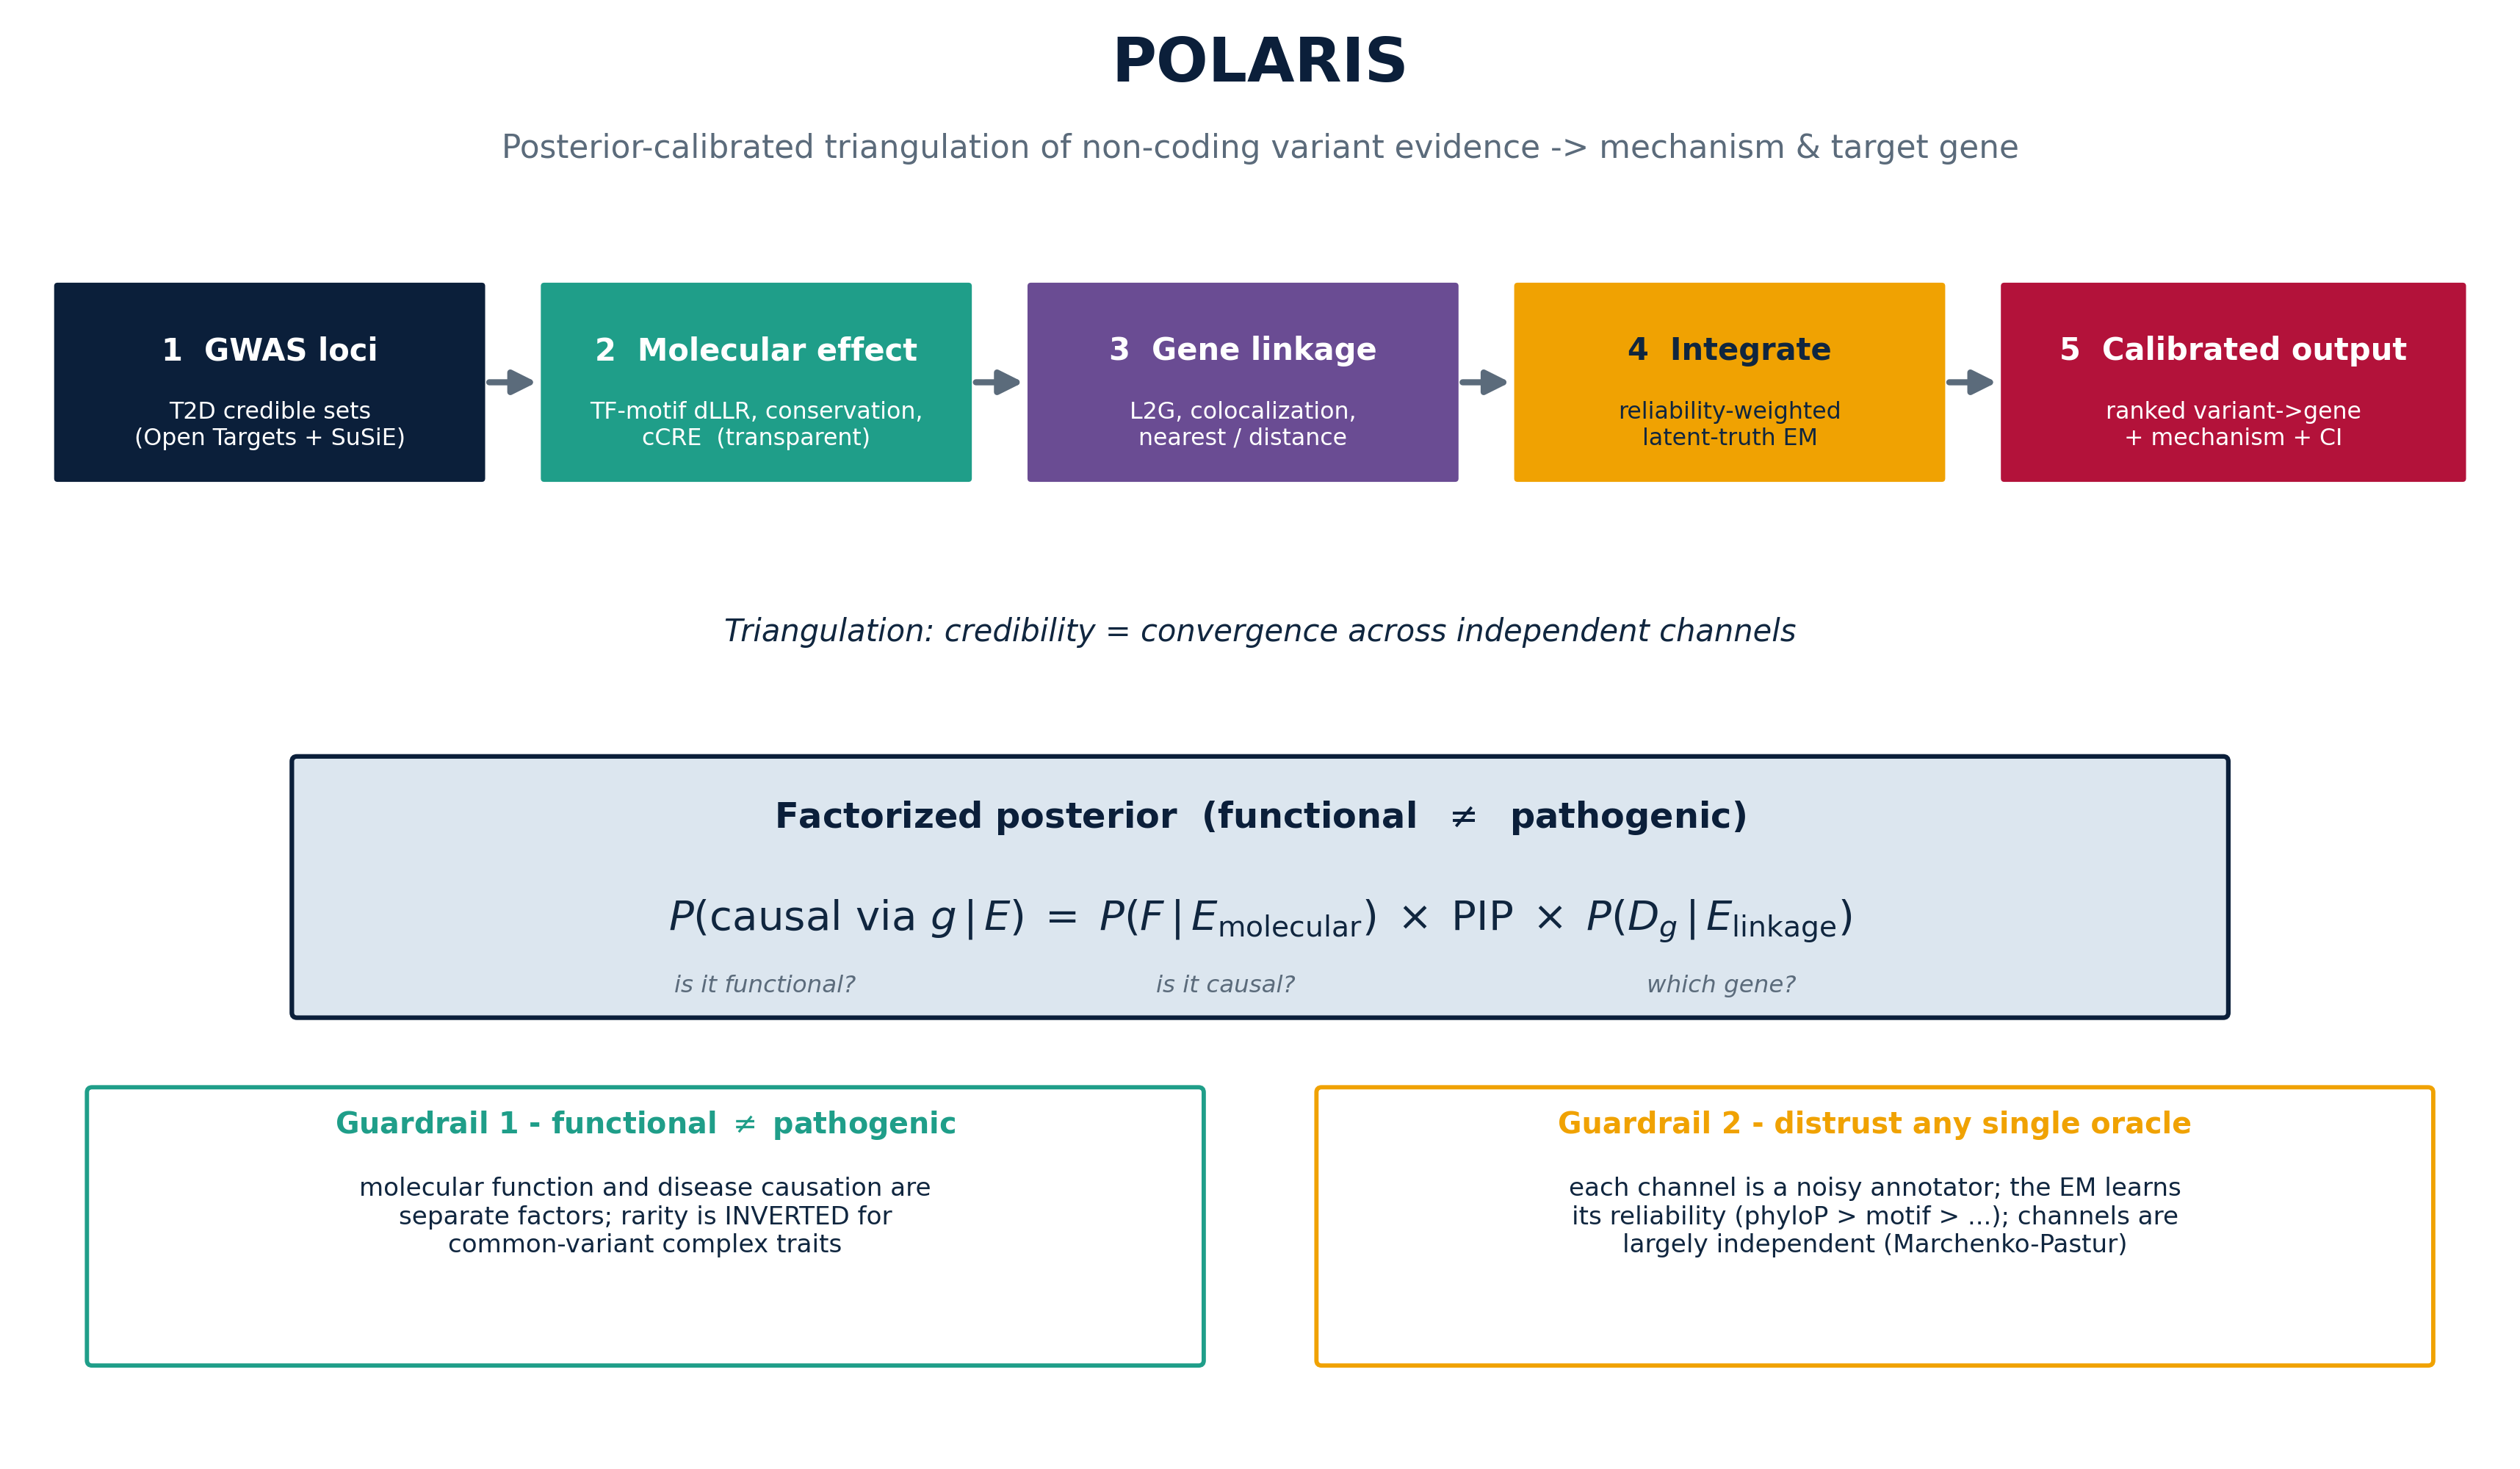
\includegraphics[width=\linewidth]{fig_pipeline.png}
\caption{\textbf{POLARIS architecture.} A six-step, fully public pipeline emits calibrated
variant$\rightarrow$gene hypotheses with transparent mechanism. The factorized posterior and the two
guardrails (functional $\neq$ pathogenic; distrust any single oracle) are made mathematical.}
\label{fig:pipeline}\end{figure}

\begin{figure}[t]\centering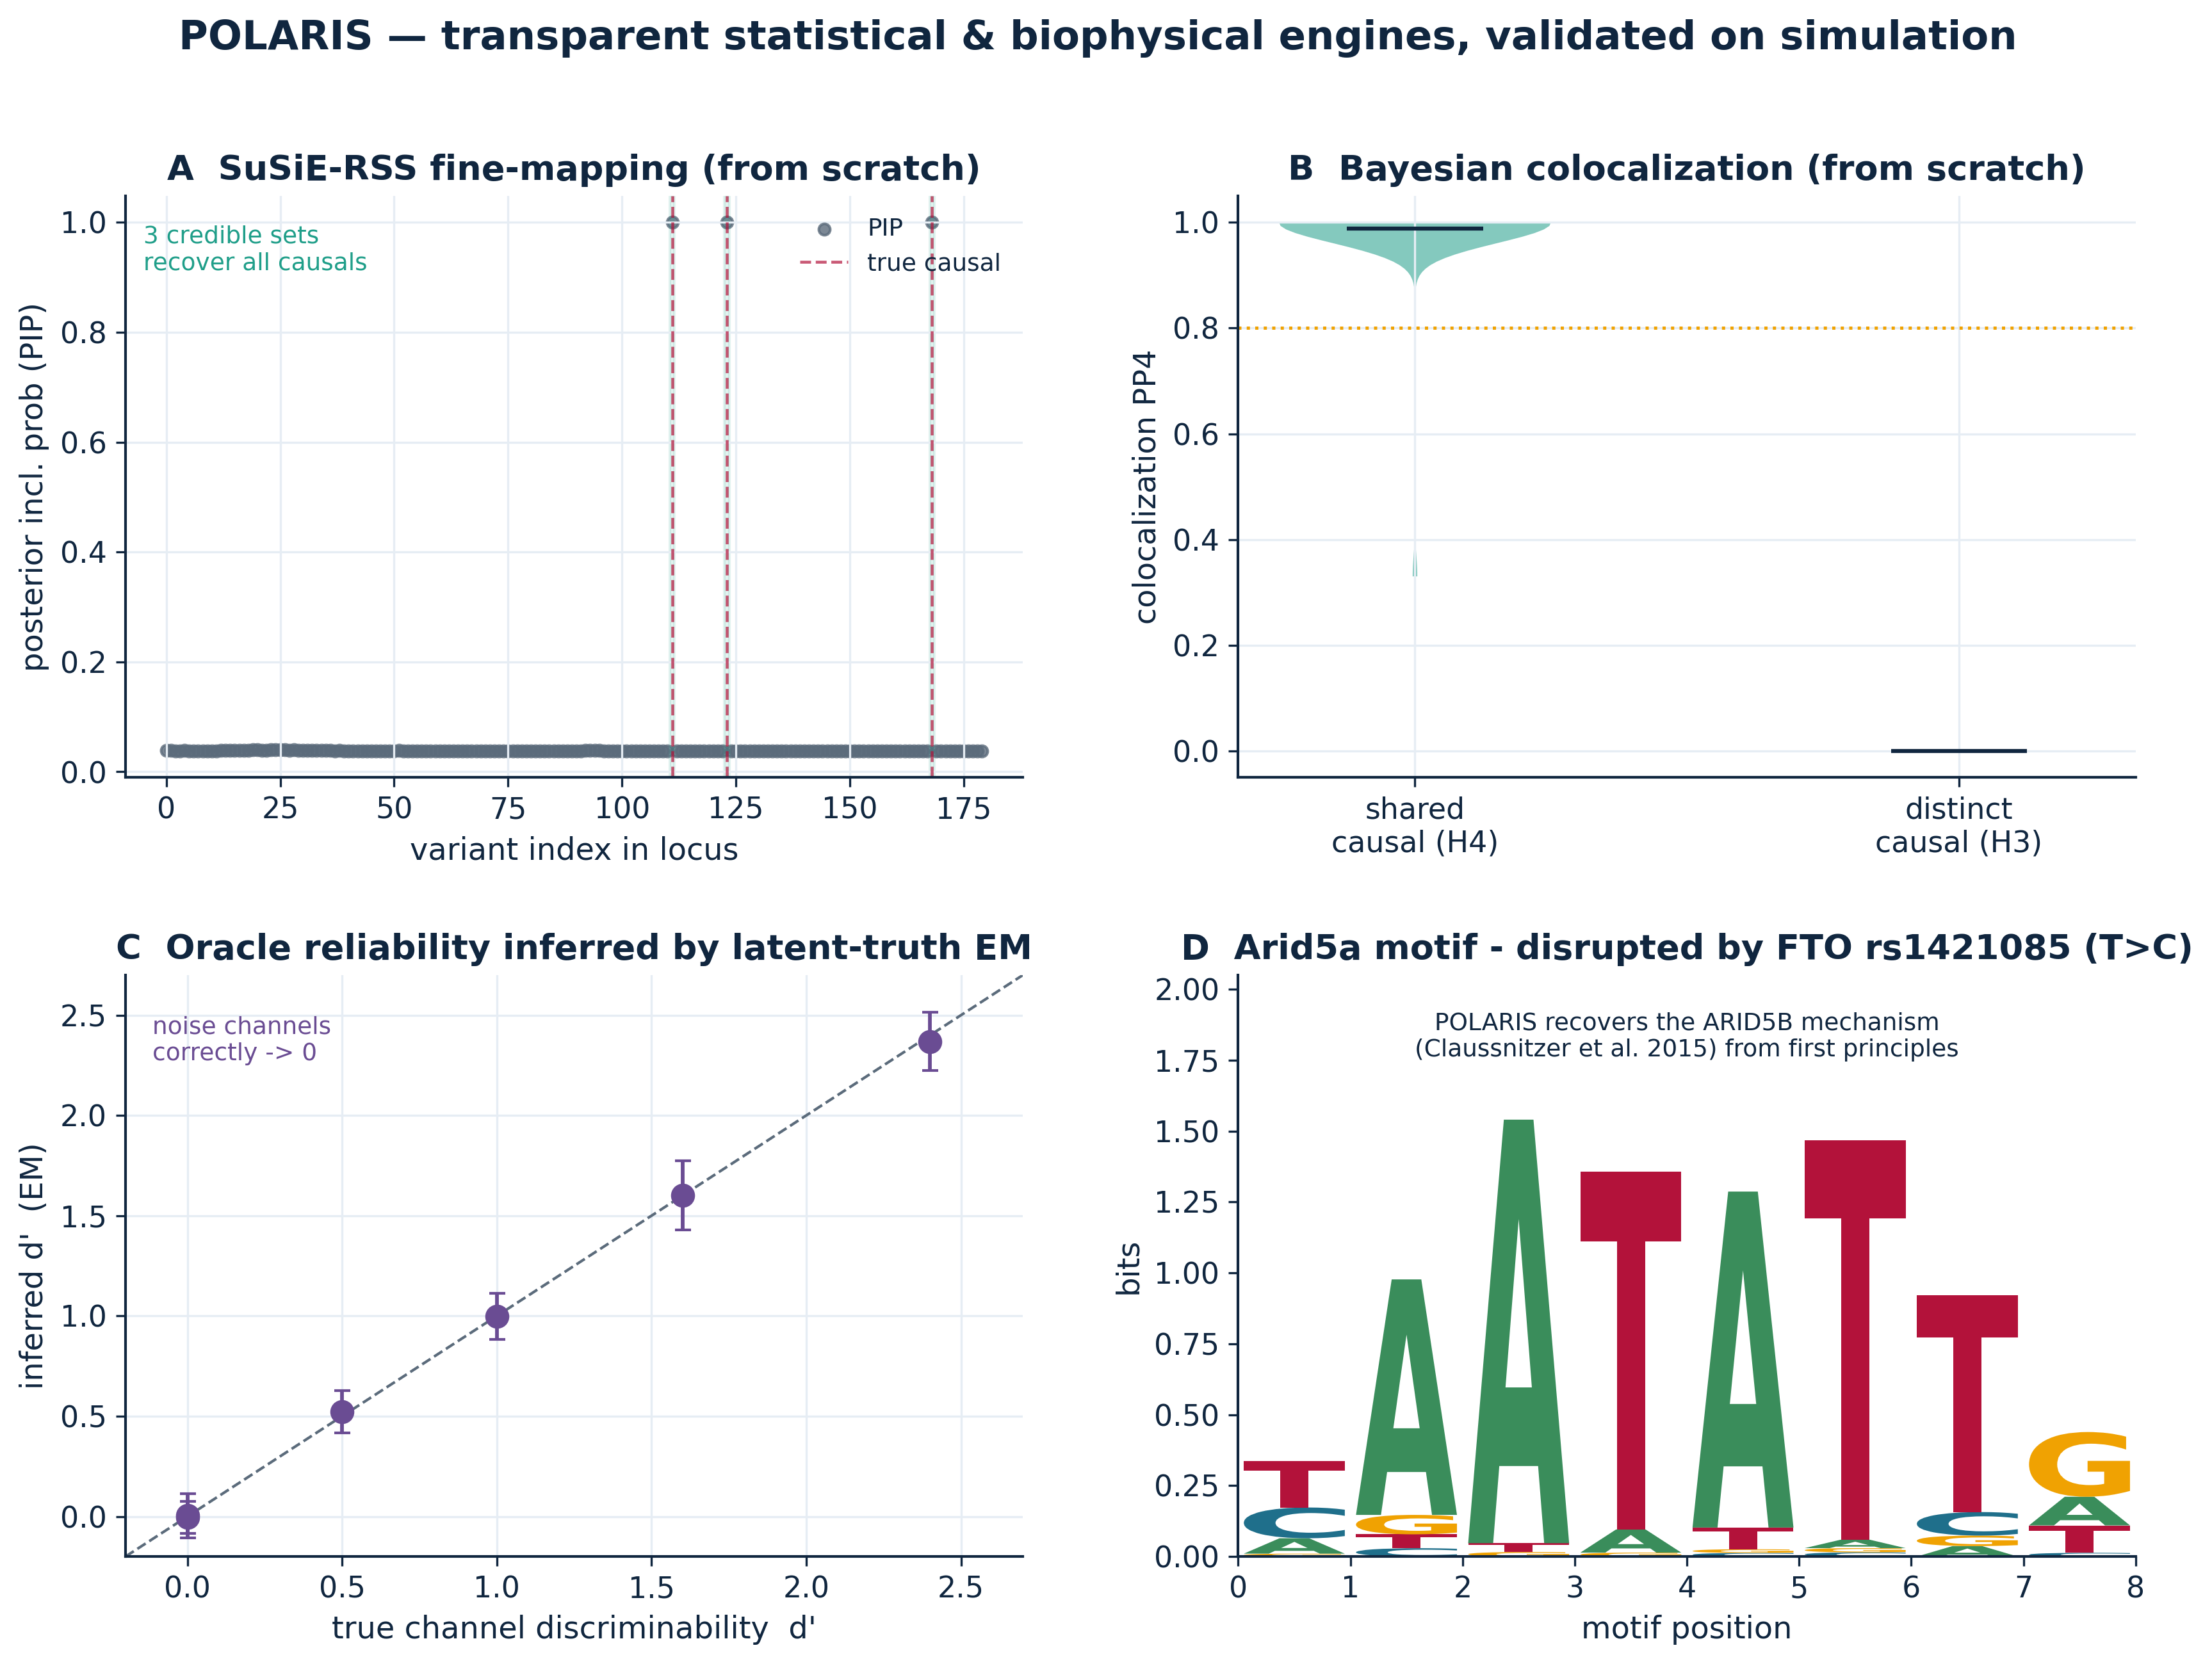
\includegraphics[width=\linewidth]{fig_methods_validation.png}
\caption{\textbf{Transparent engines, validated on simulation.} (A) From-scratch SuSiE-RSS recovers
causal variants with calibrated credible sets. (B) From-scratch Bayesian colocalization separates
shared- from distinct-causal configurations. (C) The latent-truth EM recovers true channel
discriminabilities and zeroes noise channels. (D) The information-theoretic motif logo: the ARID5B
site disrupted by \emph{FTO} rs1421085.}
\label{fig:methods}\end{figure}

\begin{figure}[t]\centering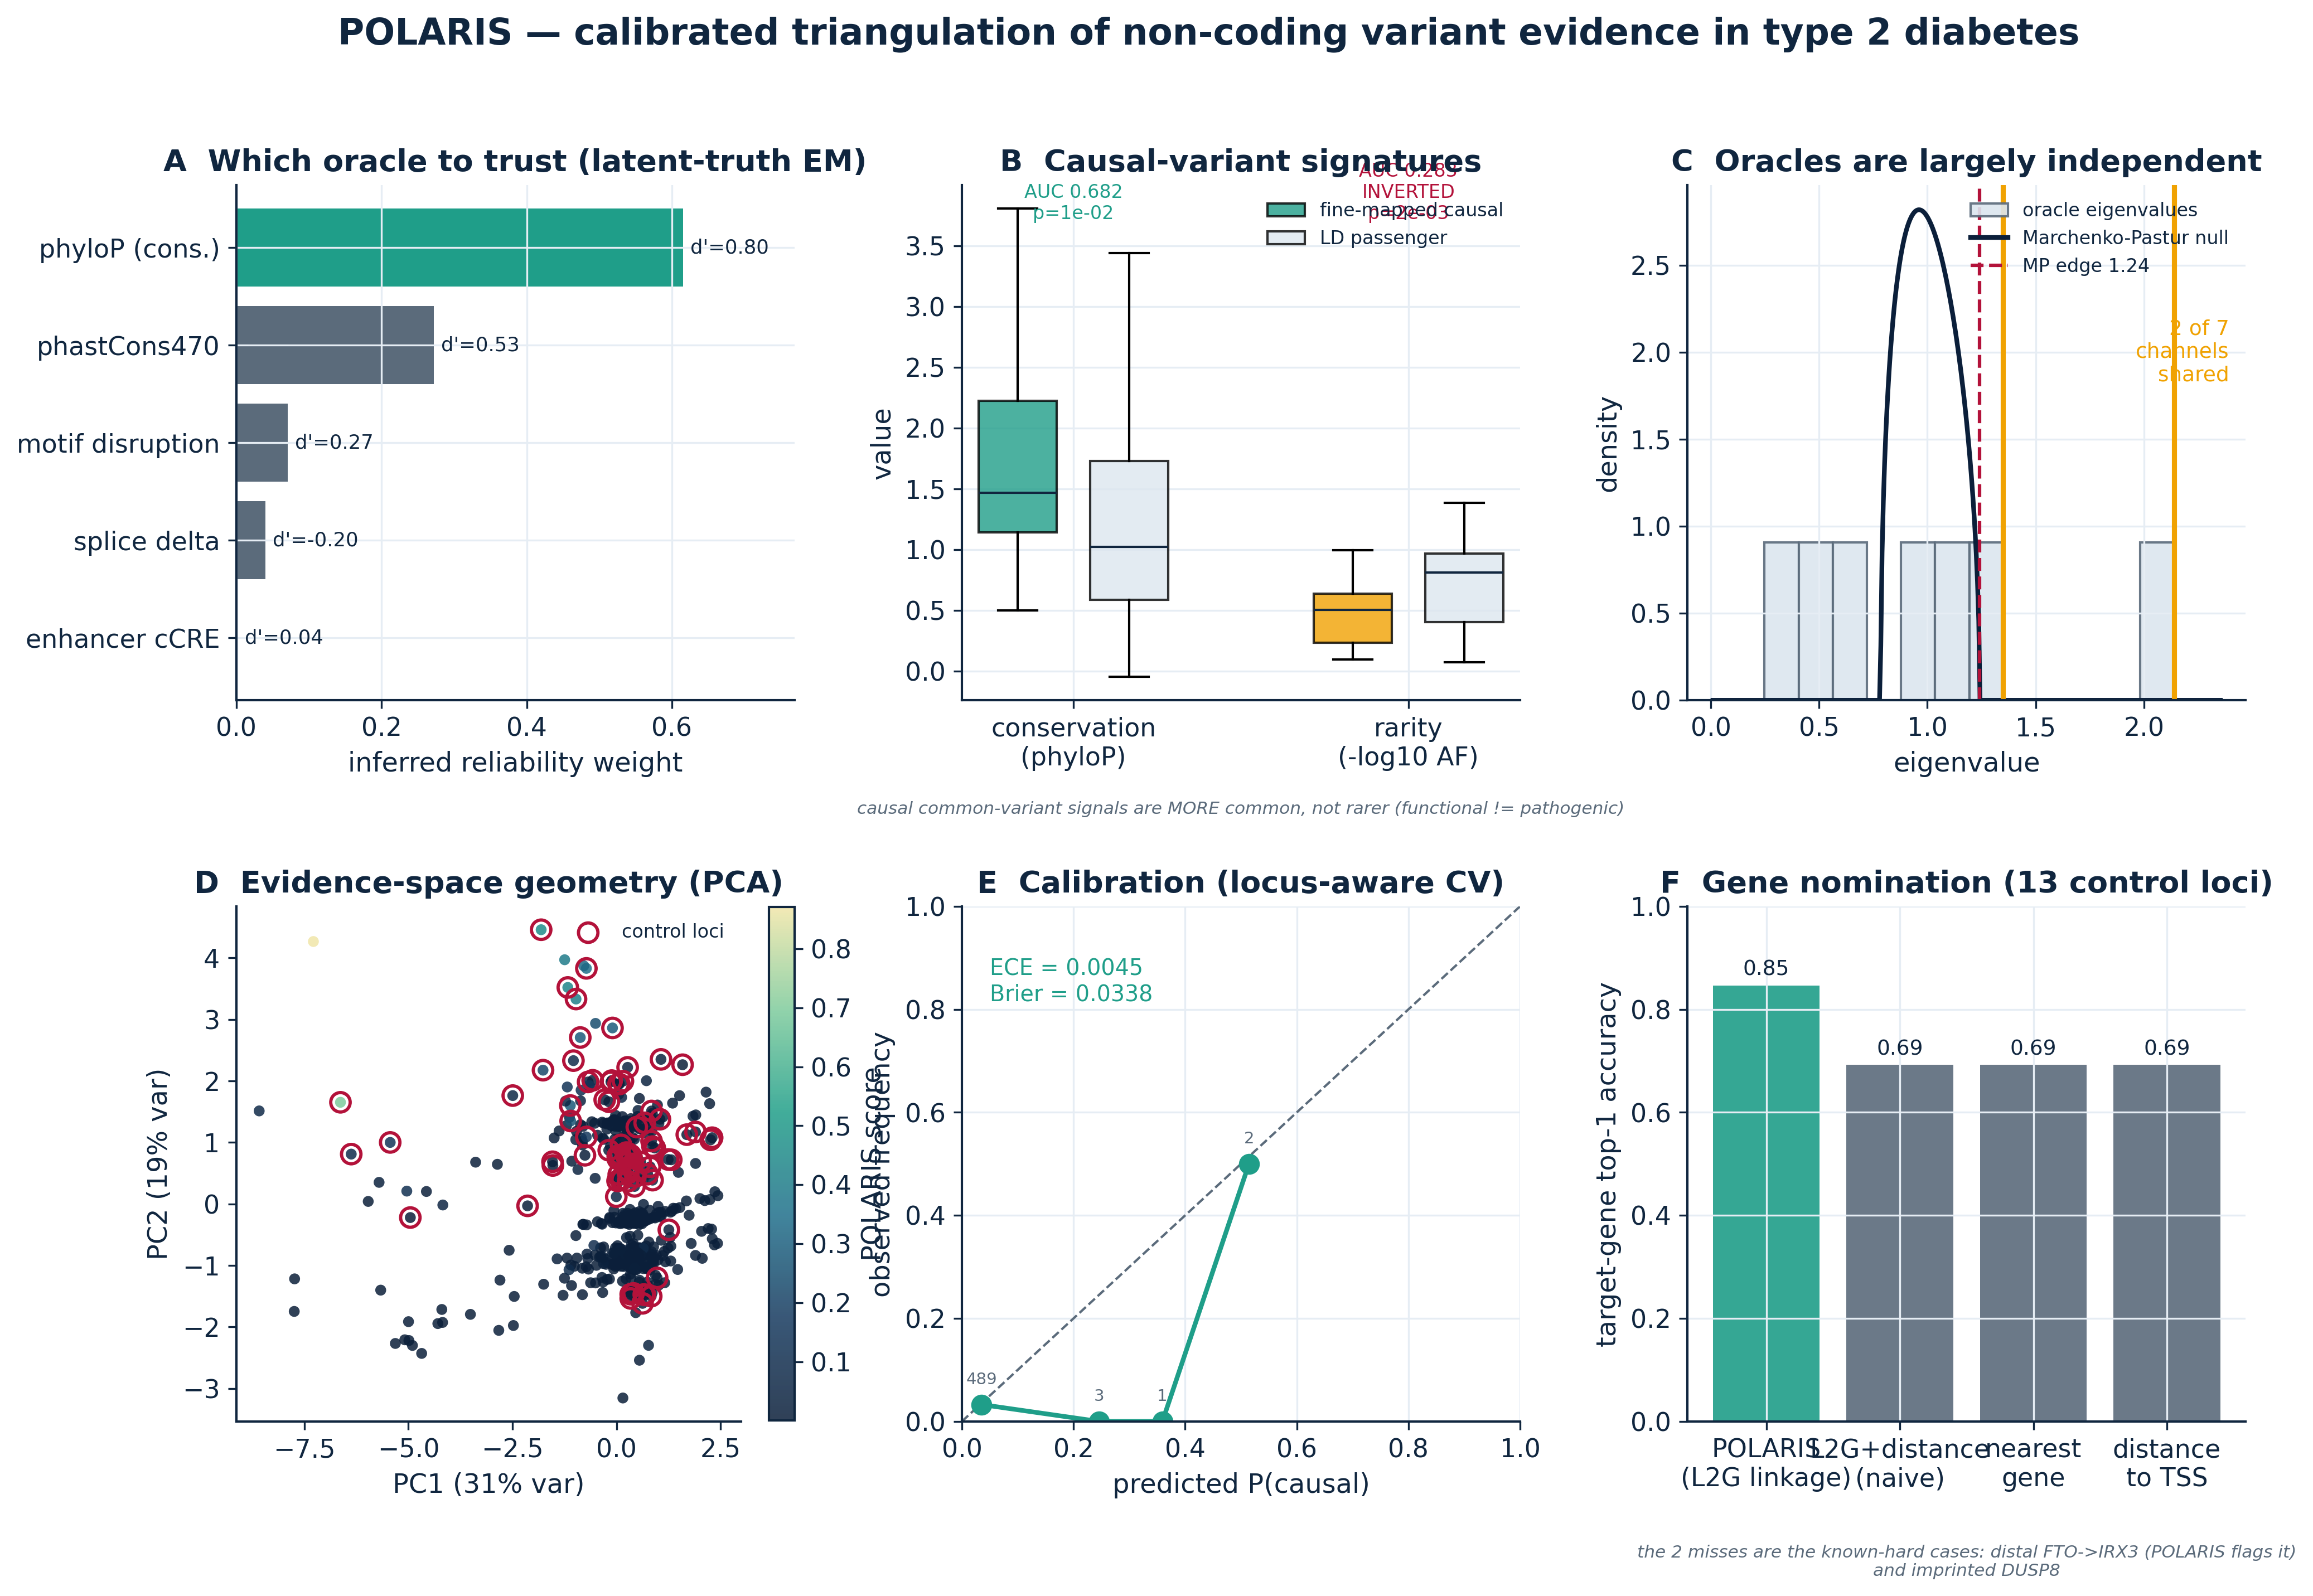
\includegraphics[width=\linewidth]{fig_results_main.png}
\caption{\textbf{Calibrated triangulation in T2D.} (A) EM-inferred channel reliability. (B) Causal
variants are more conserved (phyloP) and \emph{less} rare (rarity inverted). (C) Marchenko--Pastur null:
channels are largely independent. (D) Evidence-space geometry (PCA), coloured by POLARIS. (E) Calibration
under locus-aware CV. (F) Gene-nomination accuracy; naive distance \emph{hurts}.}
\label{fig:results}\end{figure}

\begin{figure}[t]\centering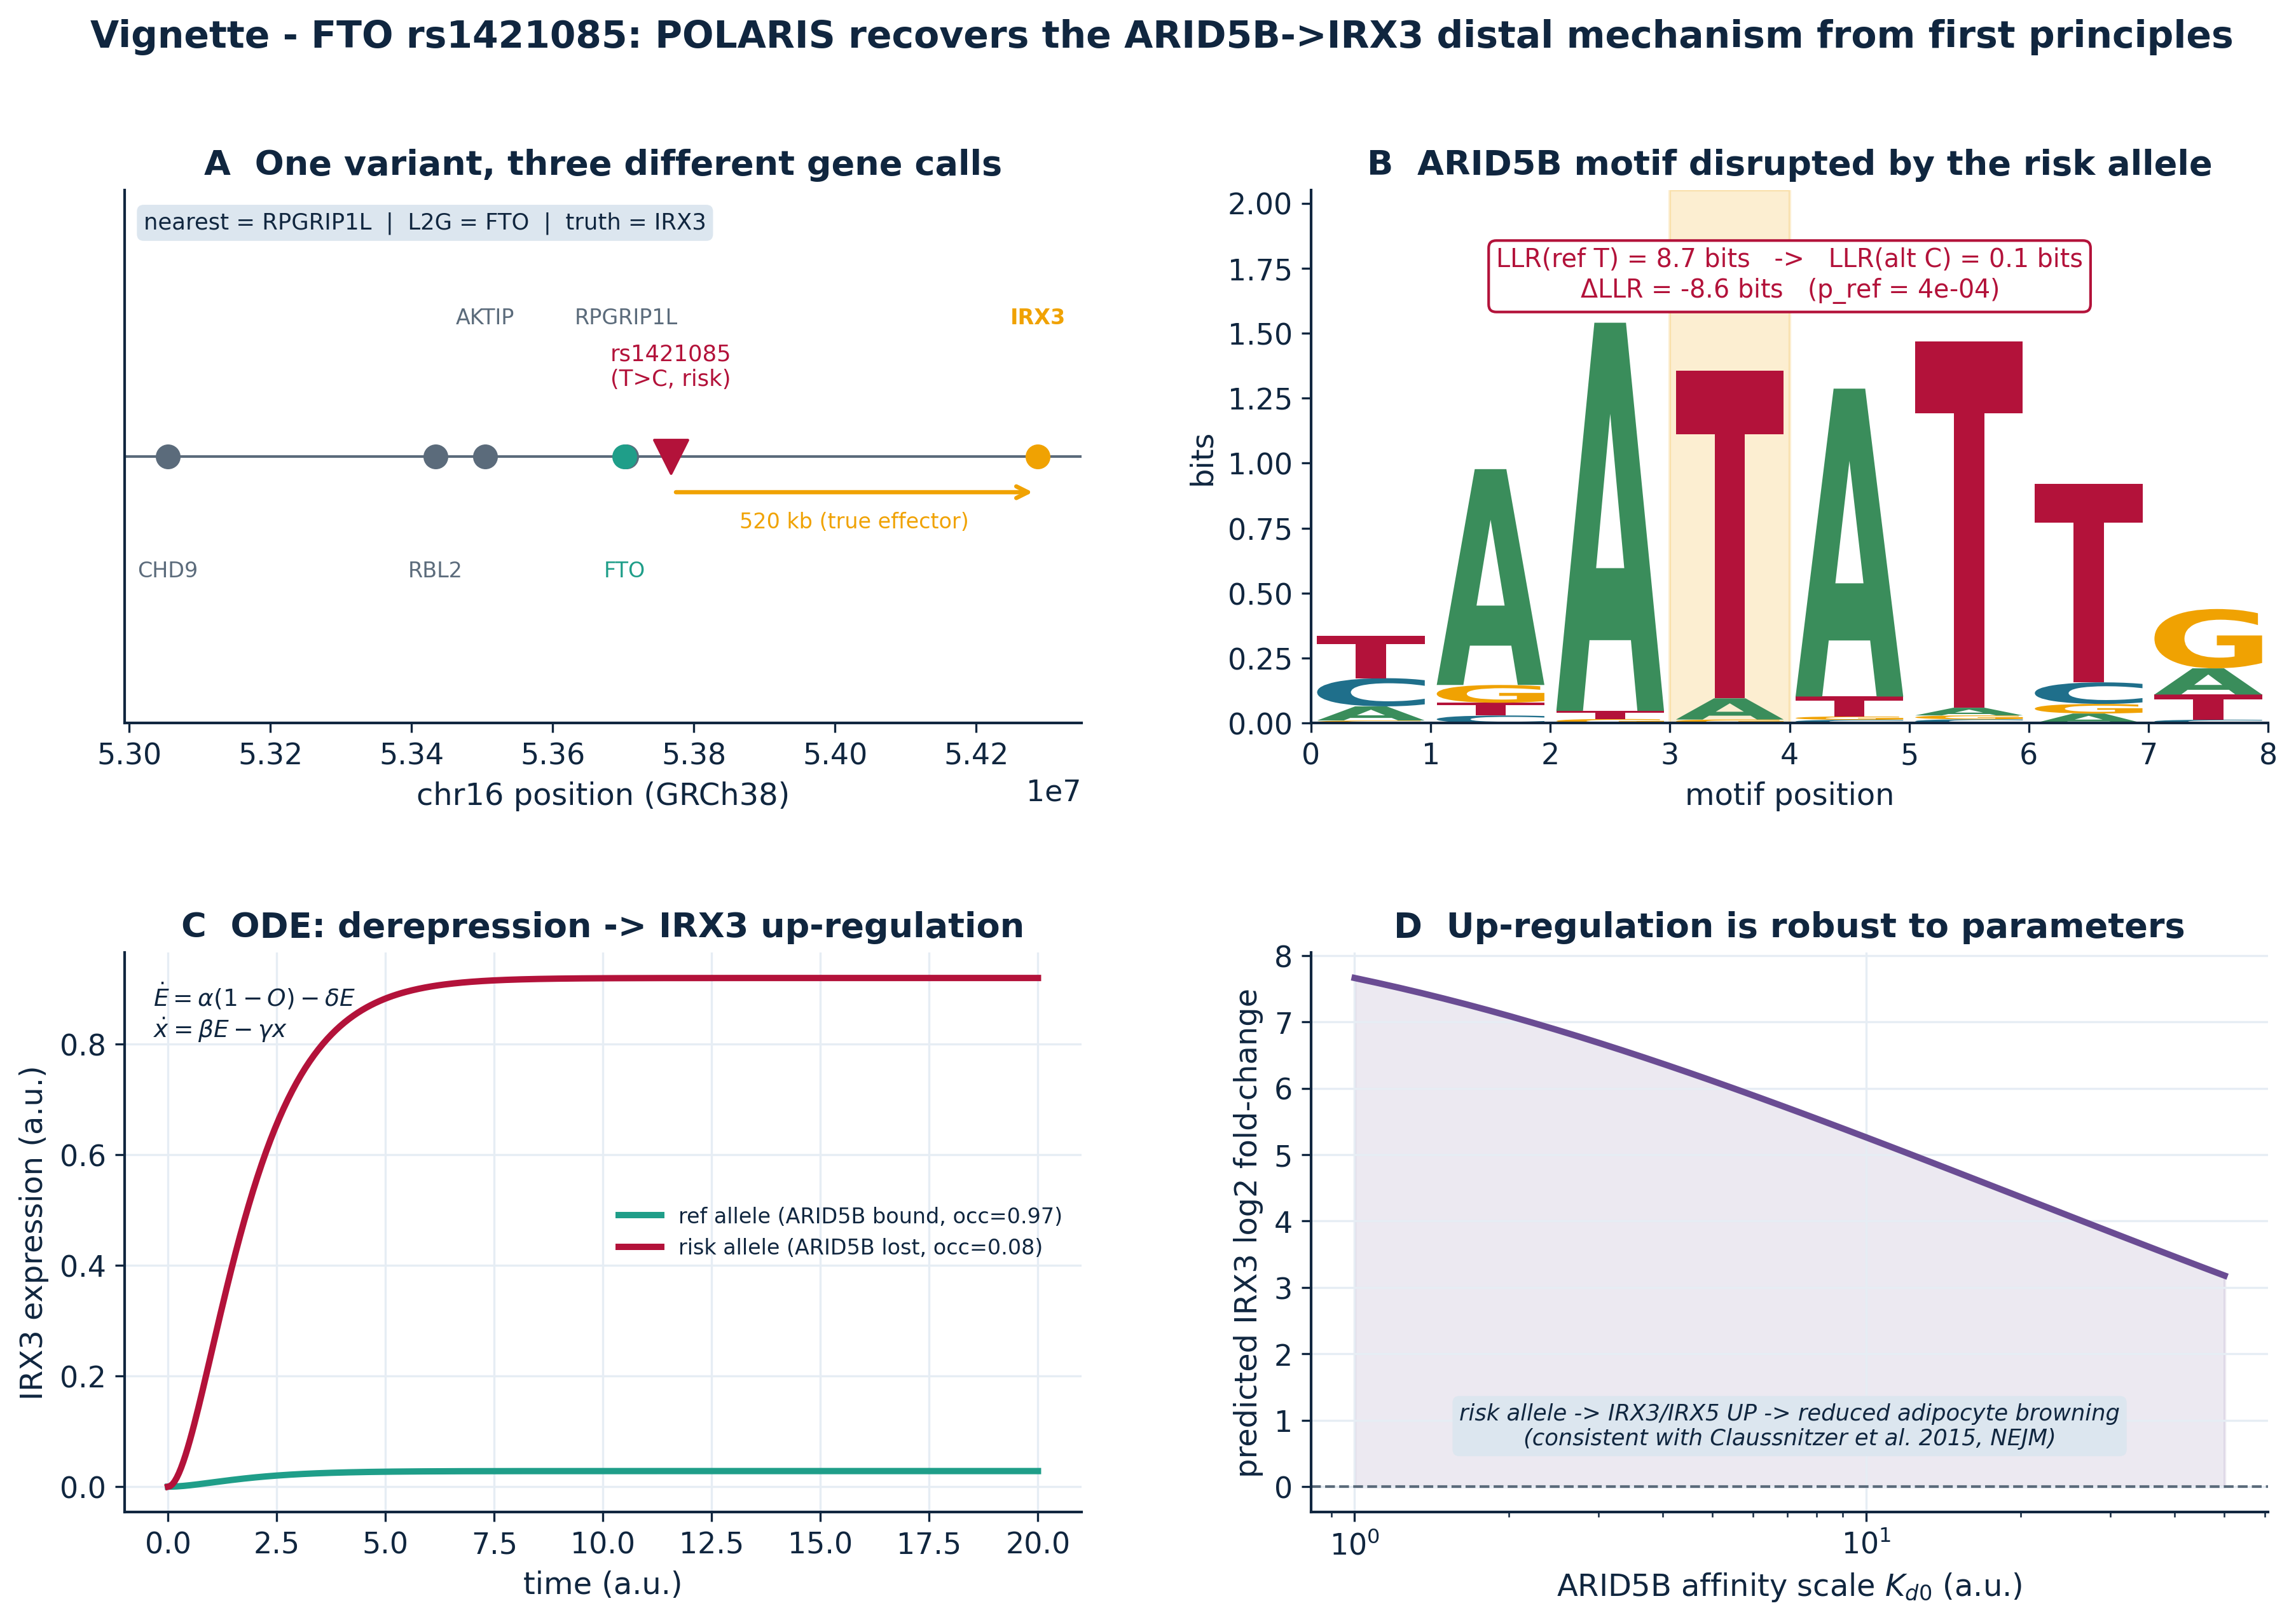
\includegraphics[width=\linewidth]{fig_vignette_fto.png}
\caption{\textbf{Vignette: \emph{FTO} rs1421085.} (A) One variant, three different gene calls. (B) The
disrupted ARID5B motif and allelic $\Delta$LLR. (C) ODE dynamics: derepression up-regulates \emph{IRX3}.
(D) The predicted direction is robust to parameters, matching \citet{claussnitzer2015fto}.}
\label{fig:vignette}\end{figure}

\begin{figure}[t]\centering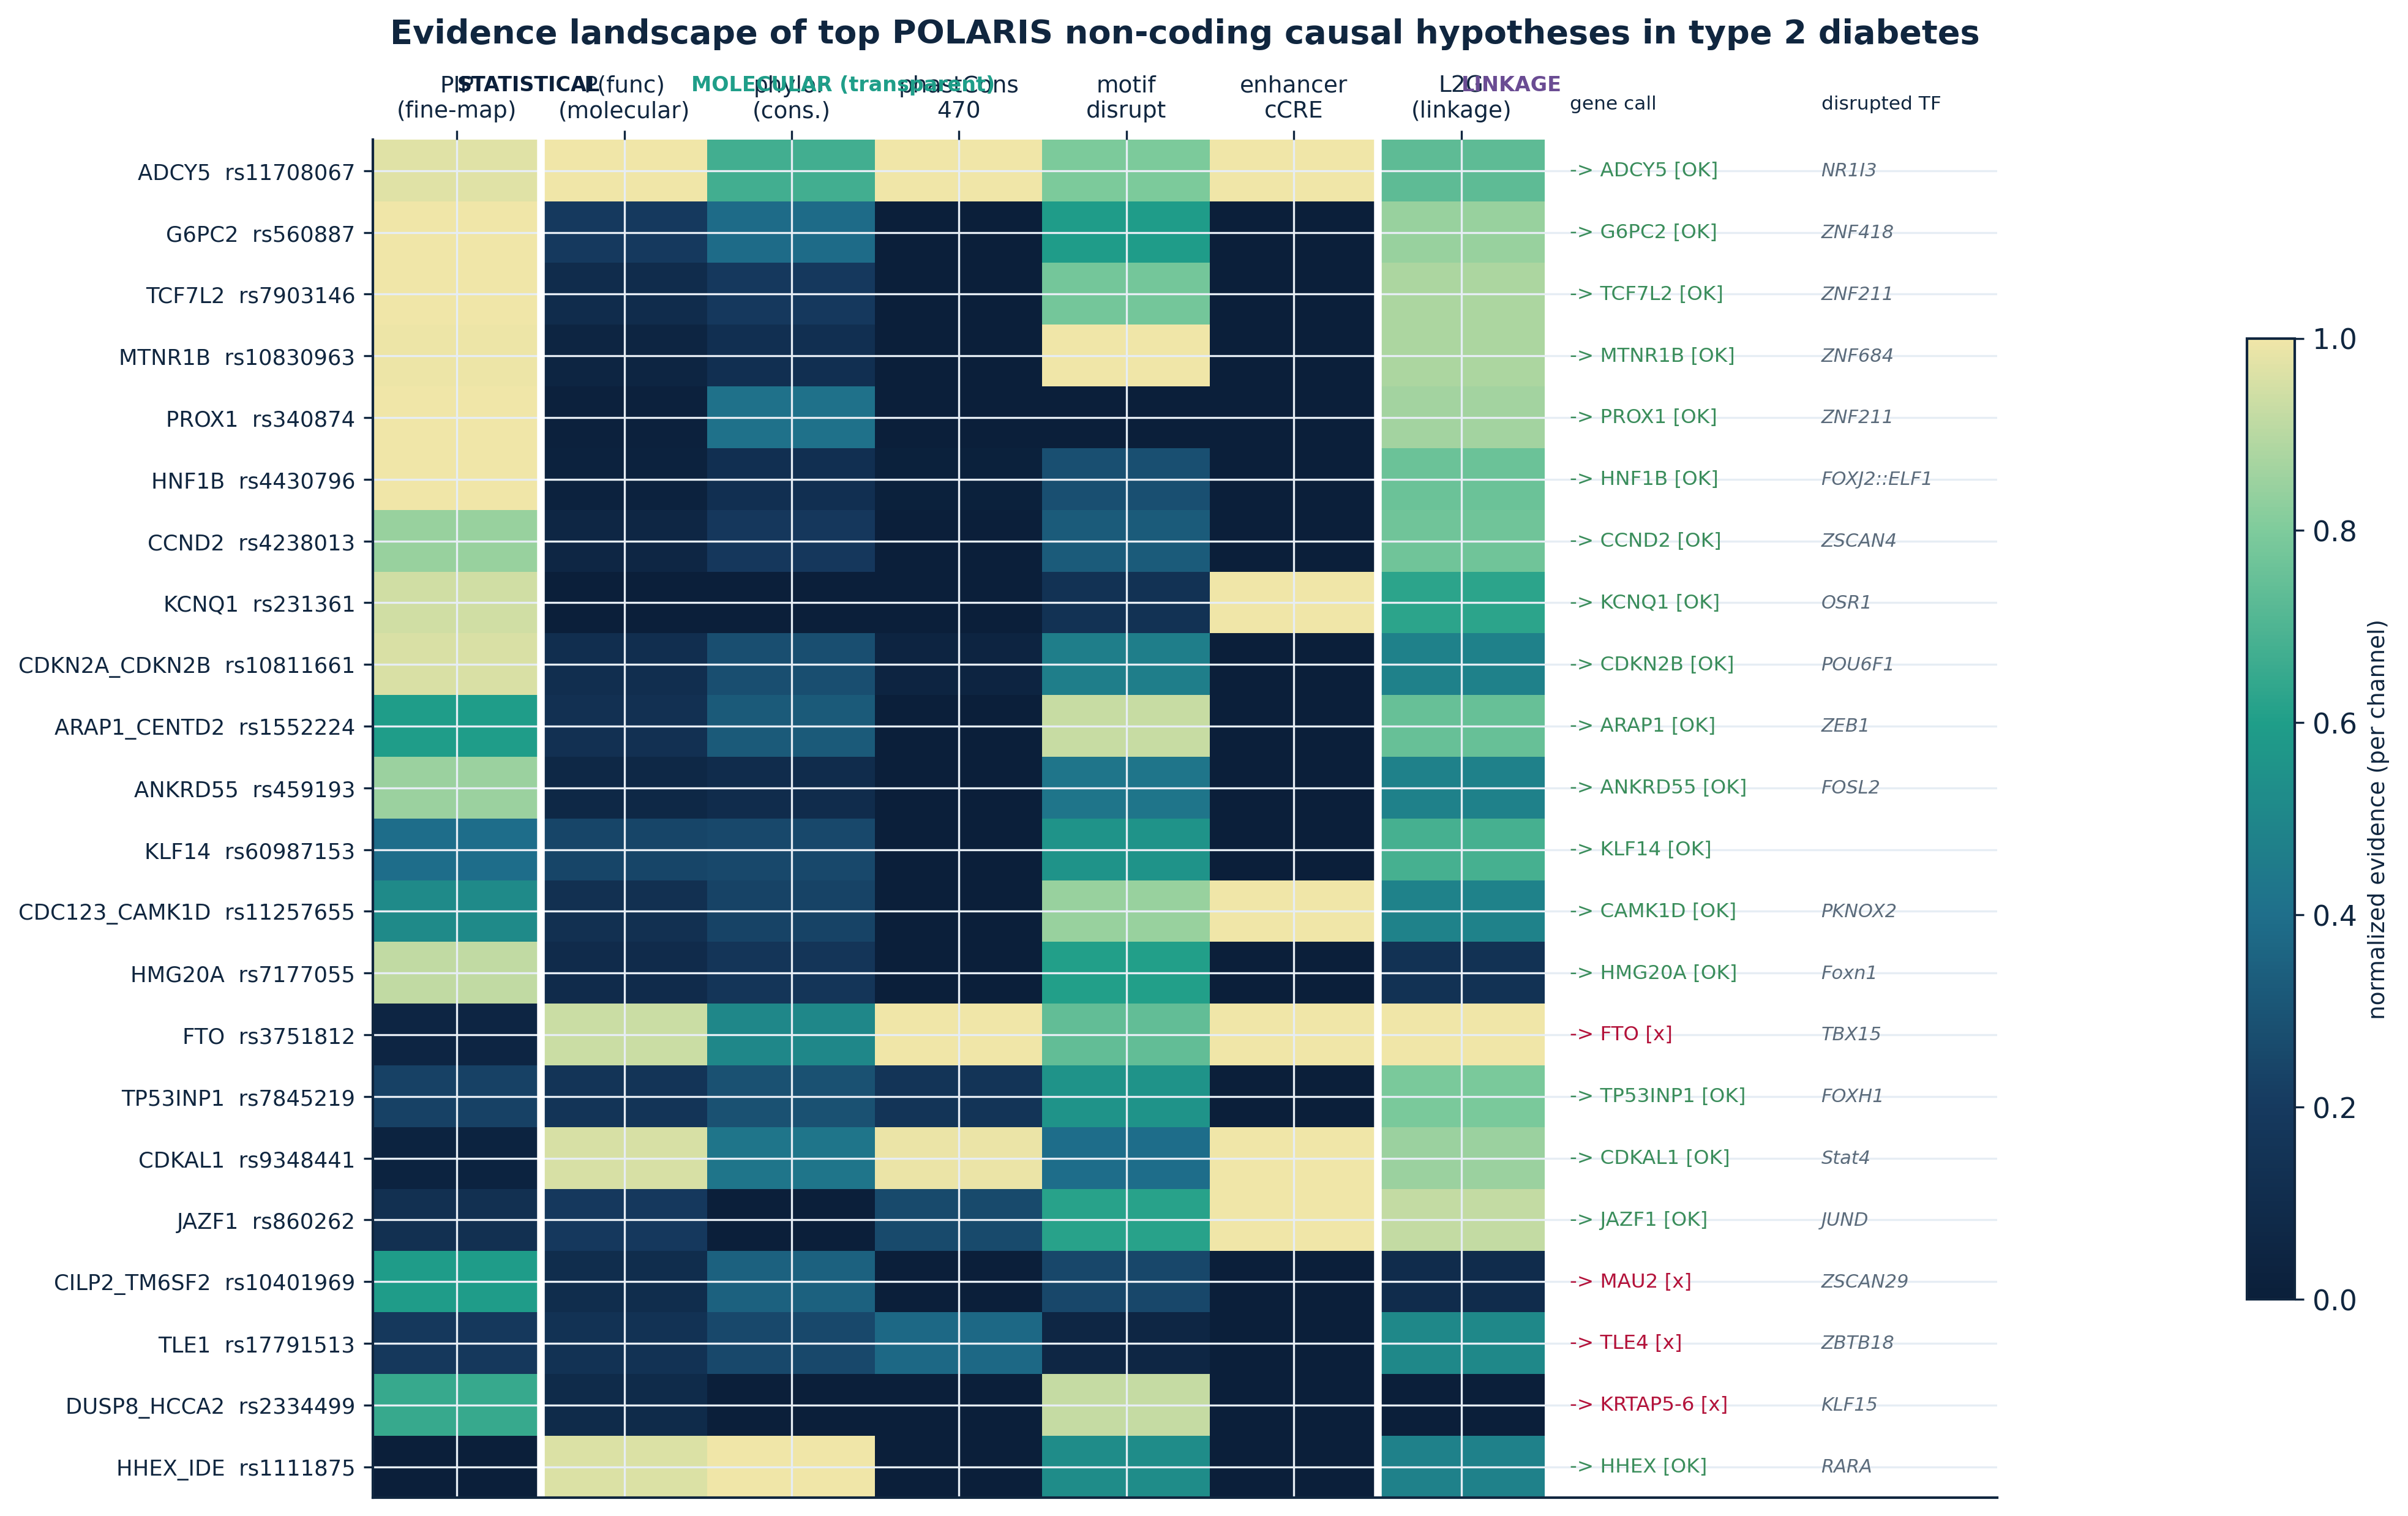
\includegraphics[width=0.92\linewidth]{fig_evidence_heatmap.png}
\caption{\textbf{Evidence landscape} of top non-coding causal hypotheses: statistical, transparent
molecular, and linkage channels, with target-gene call (hit/miss) and disrupted TF.}
\label{fig:heatmap}\end{figure}

\begin{figure}[t]\centering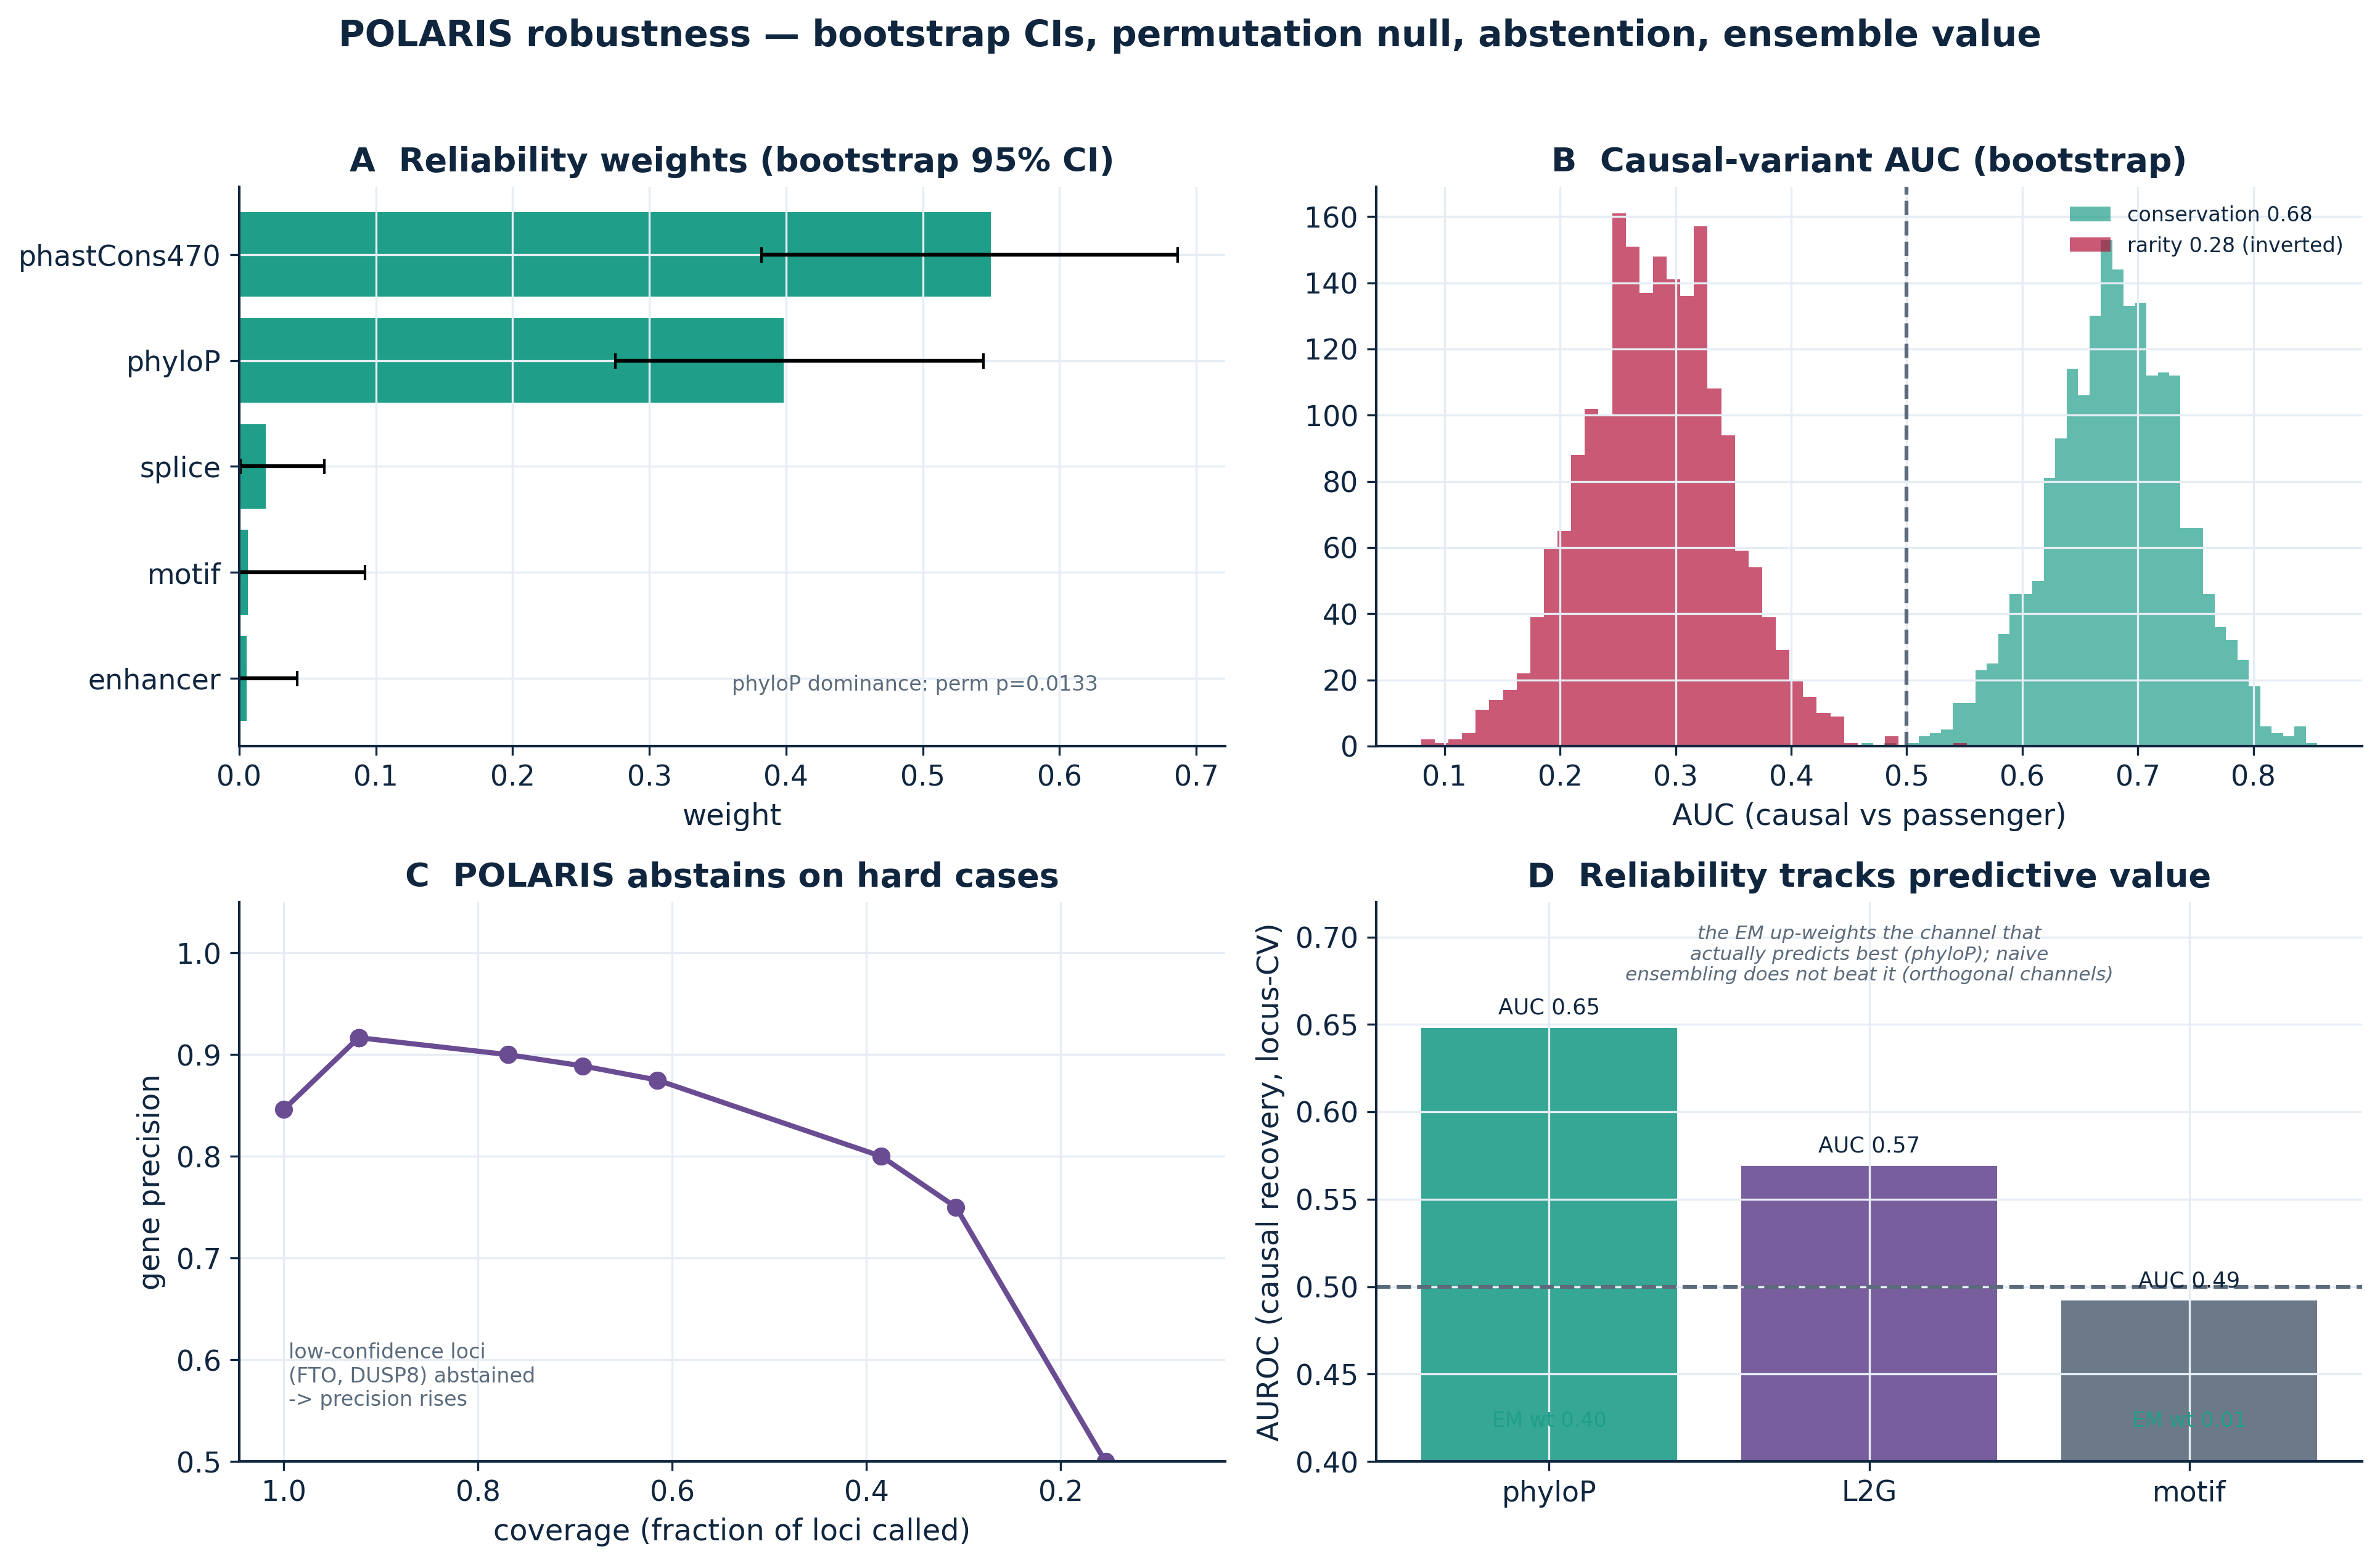
\includegraphics[width=\linewidth]{fig_robustness.png}
\caption{\textbf{Robustness.} (A) Reliability weights with bootstrap 95\% CIs. (B) Bootstrap
distributions of the conservation and (inverted) rarity AUCs. (C) Confidence-stratified abstention
raises gene precision. (D) Inferred reliability tracks predictive value; permutation $p=0.013$.}
\label{fig:robust}\end{figure}

\begin{figure}[t]\centering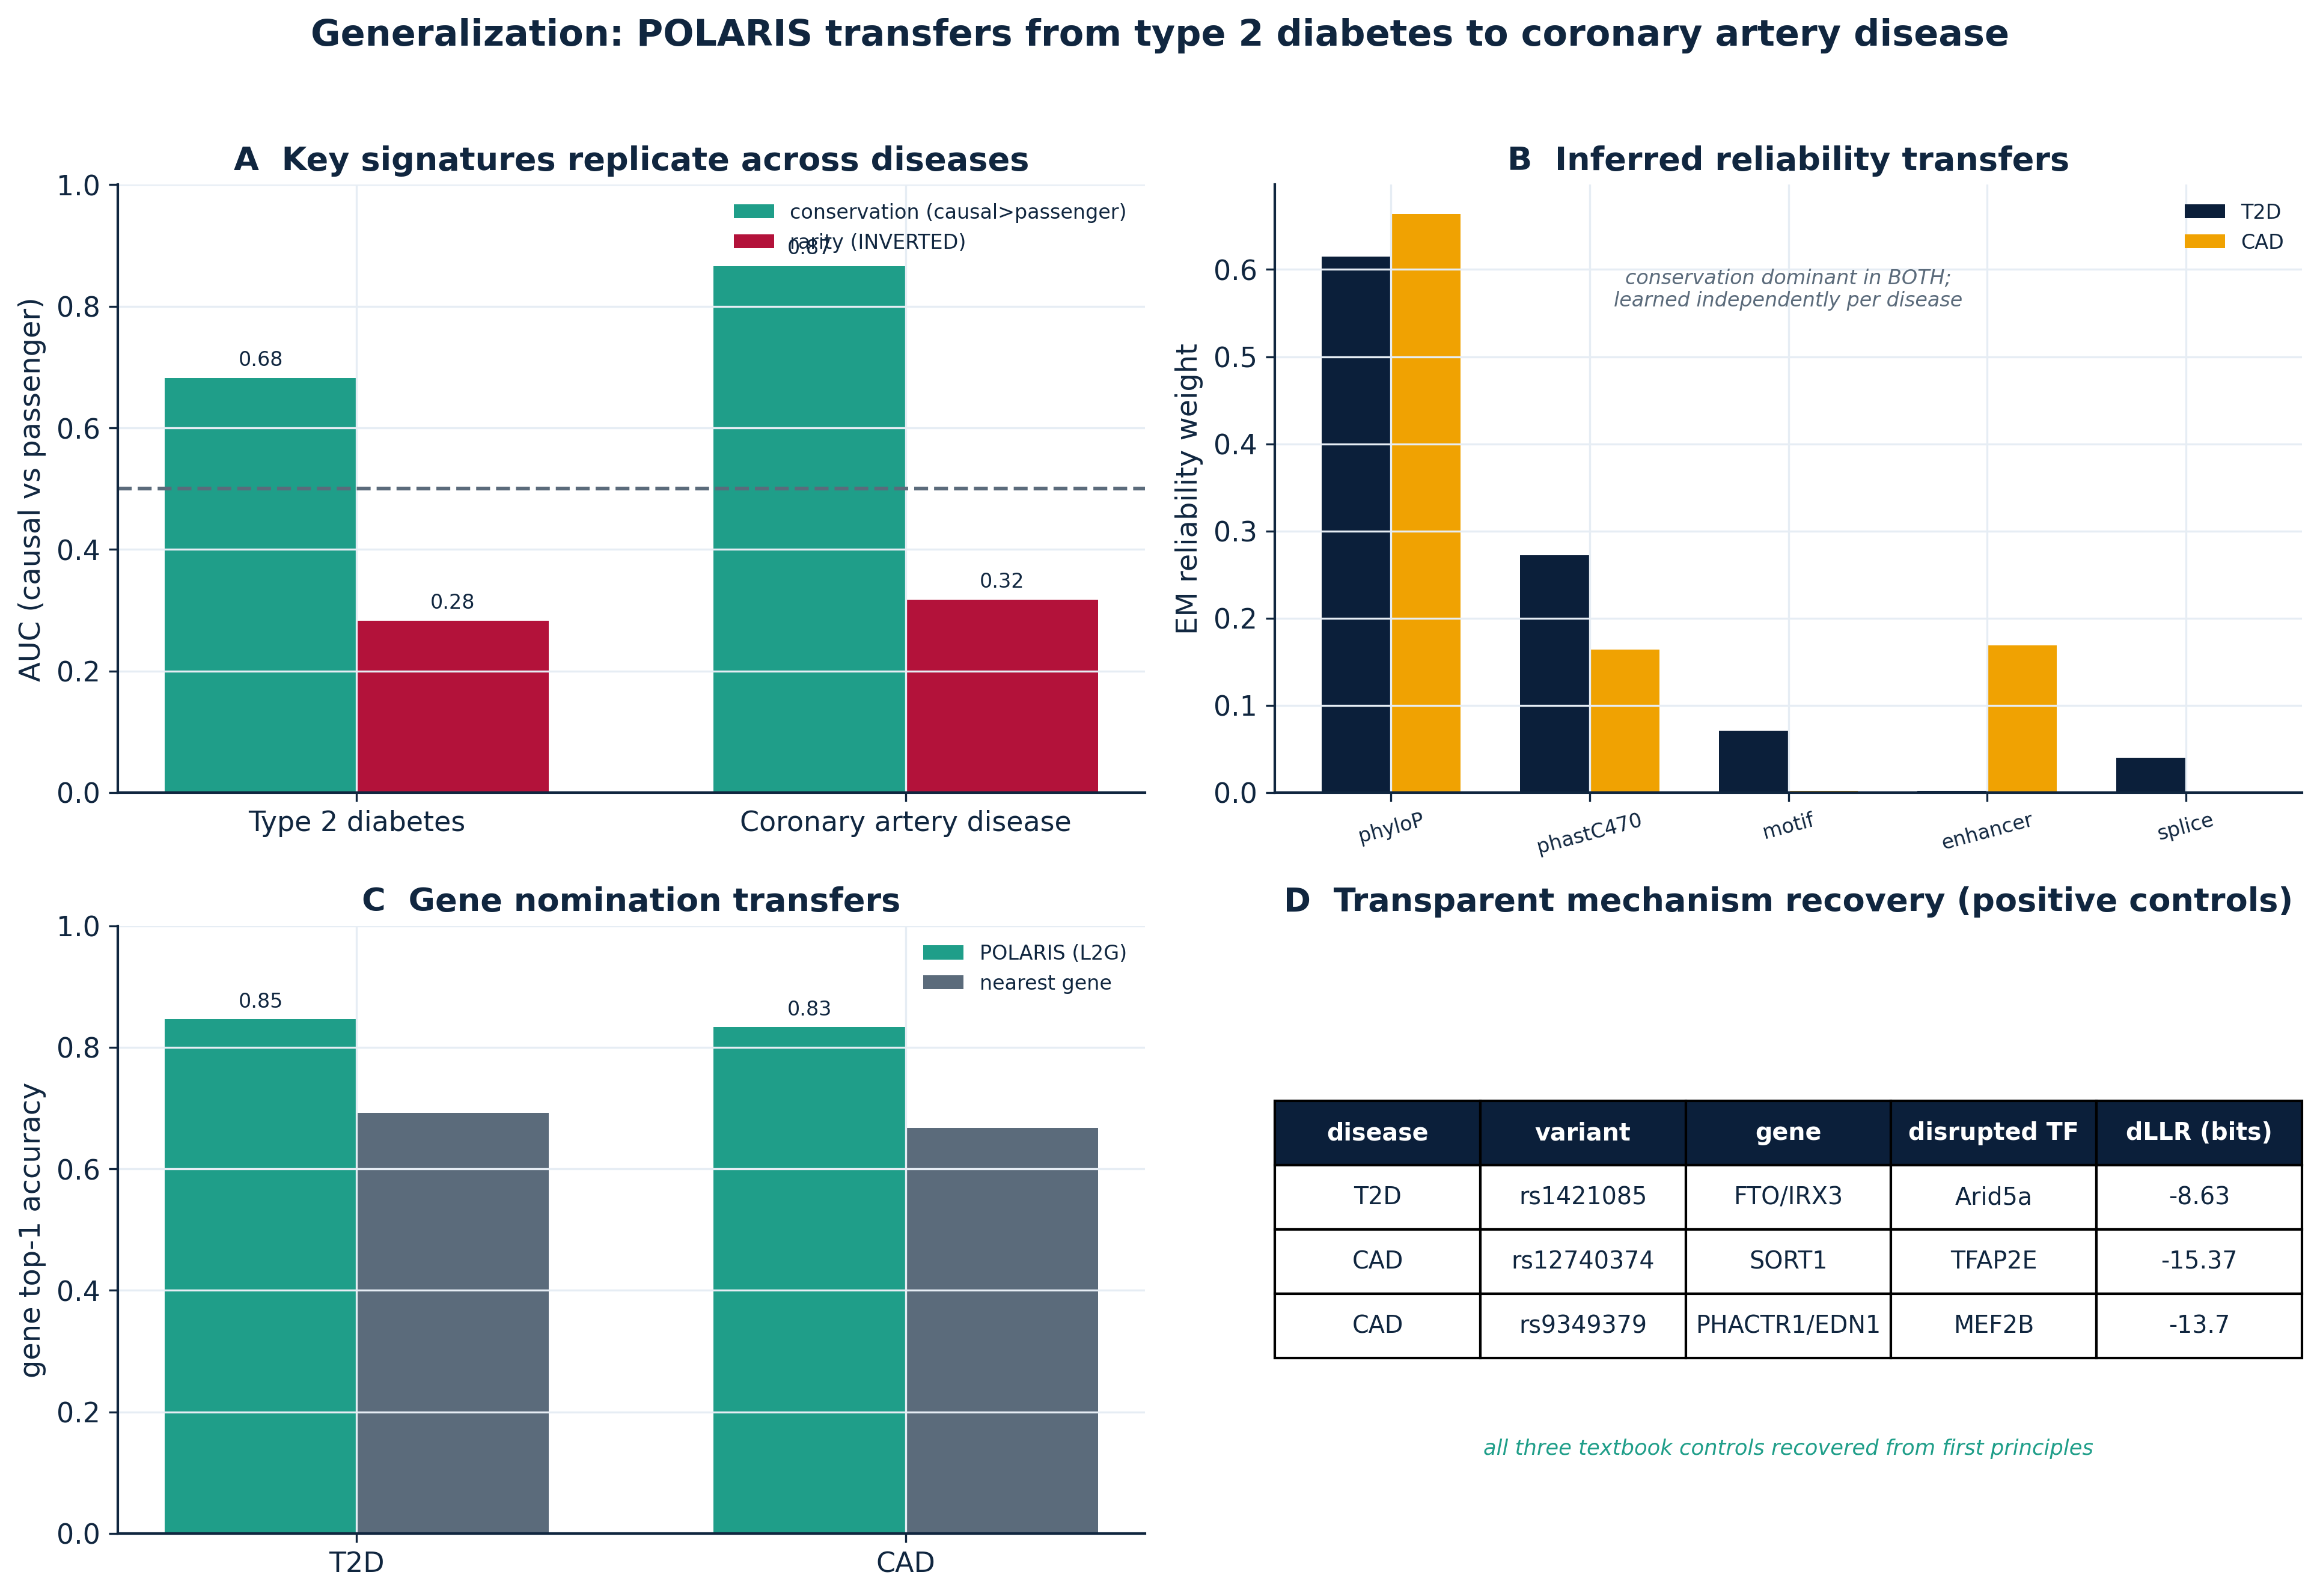
\includegraphics[width=\linewidth]{fig_generalization.png}
\caption{\textbf{Generalization, T2D$\rightarrow$CAD.} (A) Conservation enrichment and rarity inversion
replicate. (B) The EM independently re-learns the same reliability ordering. (C) Gene nomination transfers.
(D) Textbook controls (\emph{FTO/IRX3}, \emph{SORT1}, distal \emph{PHACTR1}) recovered from first
principles.}\label{fig:gen}\end{figure}

\clearpage
{\small\bibliographystyle{abbrvnat}\bibliography{polaris}}
\end{document}
